\section{Evaluation}\label{sec:evaluation}

\begin{figure*}
    \centering
    \begin{subfigure}{0.49\textwidth}
        \centering
        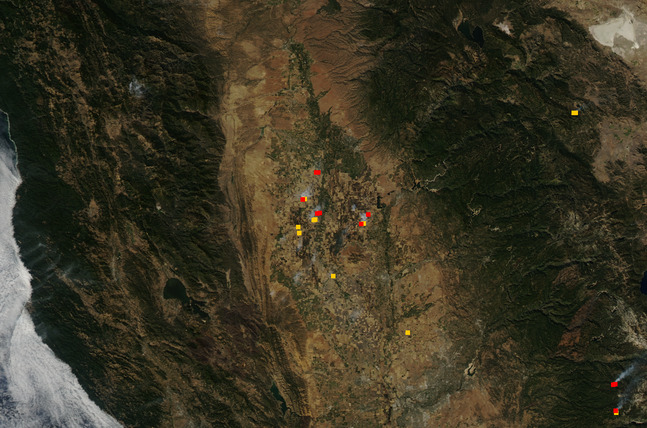
\includegraphics[width=\textwidth]{diagrams/injection/original.jpg}
        \caption{Original image with some fires.\newline}
        \label{fig:injection-orig}
    \end{subfigure}
    \begin{subfigure}{0.49\textwidth}
        \centering
        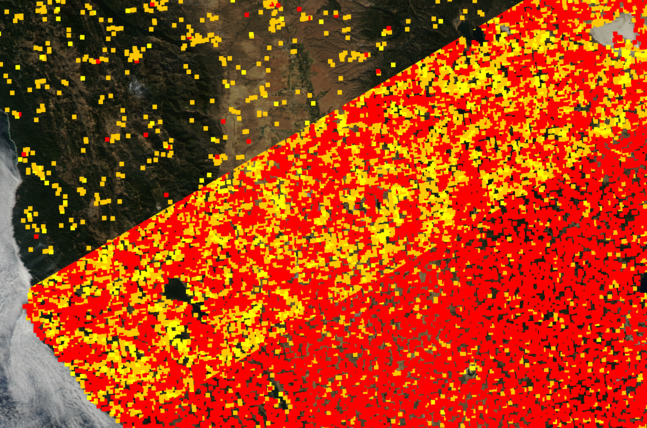
\includegraphics[width=\textwidth]{diagrams/injection/random_combined_diagonal.jpg}
        \caption{Fires randomly injected uniformly across the map. Composite of 3 images, with intensity of the fires increasing from top to bottom.}
        \label{fig:injection-random}
    \end{subfigure}
    \caption{An overview of the possible ways an attacker can manipulate the output of the forest fire detection algorithm by overshadowing the downlinked data. In each image, forest fires detected by the algorithm are highlighted in yellow, orange, and red in increasing order of intensity.}
    \label{fig:injection}
\end{figure*}

\begin{figure}
    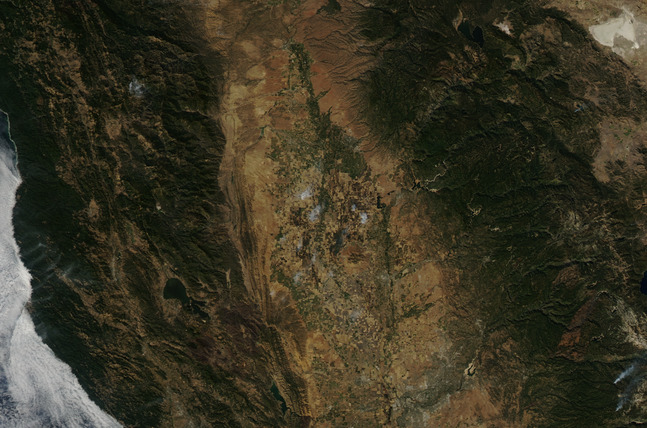
\includegraphics[width=\columnwidth]{diagrams/injection/masked_0.jpg}
    \caption{MODIS image with legitimate fires masked out.}
    \label{fig:injection-masked}
\end{figure}

Successfully injecting the signal relies upon the attacker's gain at the receiver being a certain proportion higher than the victim signal.
This proportion, known as the overshadow ratio, is dependent upon protocol level factors such as the modulation scheme and error correcting ability of the checksum.

\subsection{Dataset poisoning}

\subsubsection{Case Study: Injecting ficticious forest fires}

\subsubsection{Case Study: Masking existing forest fires}

\subsubsection{Case Study: Exploiting IPOPP image decoding}
\textbf{TODO: IPOPP Security Audit}

\subsection{Determining the overshadow ratio}
